\documentclass[11pt]{article}
\usepackage{geometry}                % See geometry.pdf to learn the layout options. There are lots.
\geometry{letterpaper}                   % ... or a4paper or a5paper or ... 
%\geometry{landscape}                % Activate for for rotated page geometry
%\usepackage[parfill]{parskip}    % Activate to begin paragraphs with an empty line rather than an indent
\usepackage{graphicx}

\title{Brief Article}
\author{The Author}
%\date{}                                           % Activate to display a given date or no date

\begin{document}
\maketitle

\tableofcontents

\pagebreak

\section{Introduction}

This is the first section
\subsection{Fourier Transform}


This is the first subsection. It contains the Fourier transform\cite{bracewell1986fourier}.

\begin{equation}
\hat{f}(\xi) = \int_{-\infty}^\infty f(x)\ e^{- 2\pi i x \xi}\,dx
\end{equation}


You can see this in Figure \ref{fig:1} on page \pageref{fig:1}.
\pagebreak
\pagebreak
\pagebreak
\pagebreak
\subsection{Justification}

Some beautifully justified text\cite{laplace1995pierre}:

In the 1820s Fourier calculated\cite{hale1971functional} that an object the size of the Earth, and at its distance from the Sun, should be considerably colder than the planet actually is if warmed by only the effects of incoming solar radiation. He examined various possible sources of the additional observed heat in articles published in 1824 and 1827. While he ultimately suggested that interstellar radiation might be responsible for a large portion of the additional warmth, Fourier's consideration of the possibility that the Earth's atmosphere might act as an insulator of some kind is widely recognized as the first proposal of what is now known as the greenhouse effect.

\begin{figure}[htp]

\centering
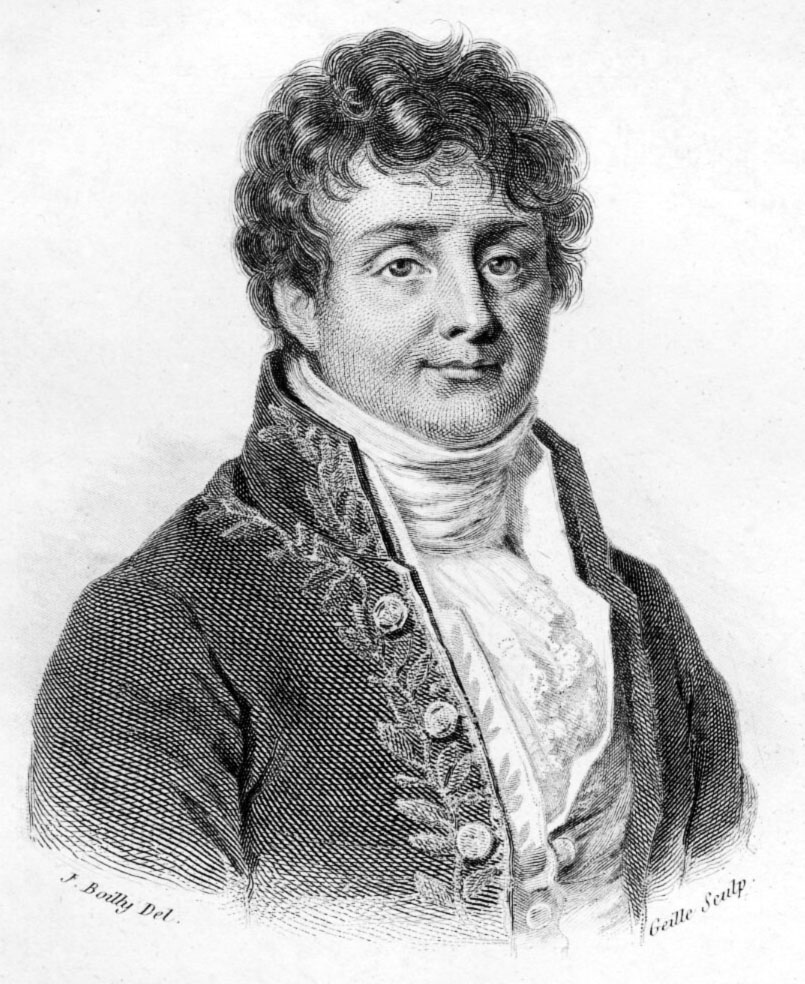
\includegraphics[width=\textwidth]{img/Fourier.jpg}
\caption{A picture of Joseph Fourier}
\label{fig:1}
\end{figure}

\bibliography{references}
	\bibliographystyle{plain}

\end{document}  